\documentclass[border=10pt]{standalone}
\usepackage{pgfplots}
\pgfplotsset{compat=1.18}
\begin{document}
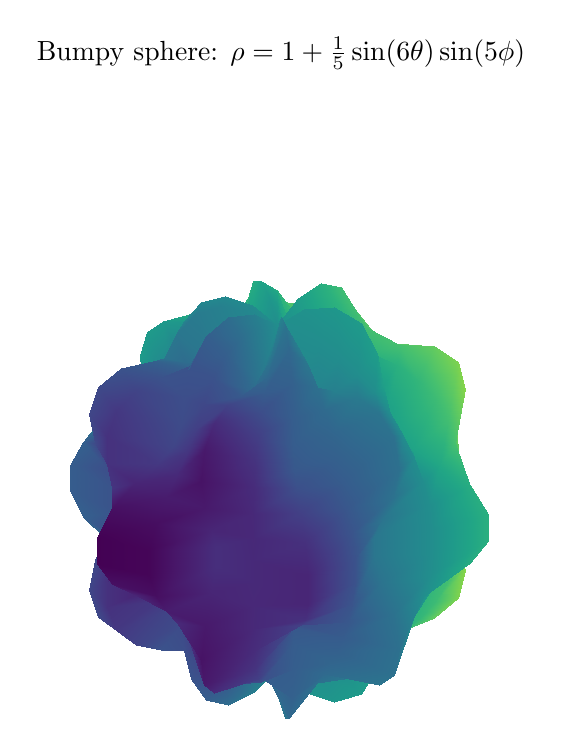
\begin{tikzpicture}
\begin{axis}[
    view={35}{25},
    axis equal image,
    axis lines=none,
    width=12cm, height=12cm,
    colormap/viridis,
    title={Bumpy sphere: $\rho = 1+\frac{1}{5}\sin(6\theta)\sin(5\phi)$},
    title style={at={(0.5,1.05)}, anchor=south},
]
\addplot3[
    surf,
    shader=interp,
    samples=24,
    samples y=24,
    domain=0:360,
    y domain=0:180,
    z buffer=sort,
    point meta={sin(180*y/180)*cos(180*x/180)},
]
    ({(1+0.2*sin(6*x)*sin(5*y))*sin(y)*cos(x)},
     {(1+0.2*sin(6*x)*sin(5*y))*sin(y)*sin(x)},
     {(1+0.2*sin(6*x)*sin(5*y))*cos(y)});
\end{axis}
\end{tikzpicture}
\end{document}